\documentclass{ctexart}
\usepackage{graphicx}
\usepackage{caption}
\usepackage{float}
\usepackage{amsmath}
\usepackage{fancyhdr}
\usepackage{xunicode-addon}
\usepackage{booktabs}
\usepackage{listings}
\usepackage{hyperref}
\usepackage[a4paper,hmargin=1.25in,vmargin=1in]{geometry}
% !TeX program = xelatex
\lstdefinestyle{mystyle}{
  basicstyle=\ttfamily\footnotesize,
  breakatwhitespace=false,         
  breaklines=true,                 
  captionpos=b,                    
  keepspaces=true,                 
  numbers=left,                    
  numbersep=5pt,                  
  showspaces=false,                
  showstringspaces=false,
  showtabs=false,                  
  tabsize=2
}

\lstset{style=mystyle}

\title{\begin{figure}[H]
	\centering 
	\includegraphics[height=7cm,width=14cm]{E:/Pictures/中科大.jpg}
	\end{figure}\Huge\textbf{数据结构实验报告3}\\\huge{二叉树的应用:哈夫曼编码和解码}}
\date{}
\punctstyle{banjiao} 
\pagestyle{fancy}
	\fancyhead[C]{\LARGE\textbf{实验报告3}}
	\fancyhead[L]{}
	\fancyhead[R]{}
	\fancyfoot[C]{\thepage}
\begin{document}
	\maketitle
	\thispagestyle{empty}
	
	\[\makebox{\Large{姓名:\underline{\makebox[5cm]{高茂航}}}}\]
	
    \[\makebox{\Large{学号:\underline{\makebox[5cm]{PB22061161}}}}\]
	
	\[\makebox{\Large{日期:\underline{\makebox[5cm]{2023年11月15日}}}}\]
	
	\clearpage

	\pagenumbering{arabic}

	\section{问题描述}

	用 huffman 压缩技术实现对任意文件的压缩和解压缩处理。
	要求对所有的文件类型(以.txt,.bmp,.mp4,.exe文件为例)进行压缩(以 1 个字节为单位进行 huffman 编码),
	压缩之后的文件后缀名为.huff。同时,对所有后缀名为.huff 的压缩文件进行解压缩。
	
	\section{算法描述}
	\subsection{数据结构}
用一个结构体数组储存霍夫曼树,数组下标为0到255的元素储存霍夫曼树的叶子节点,数组下标为255到510的元素储存霍夫曼树的其他节点。
用一个指针数组储存霍夫曼编码,数组下标为0到255的元素储存256个字符的霍夫曼编码。用一个结构体数组储存字符与编码的映射,
数组下标为0到255的元素储存256个字符与编码的映射。用一个长整型数组储存每个字符的权重,数组下标为0到255的元素储存256个字符的权重。
用一个长整型变量储存文件大小(字节数)。
	\subsection{程序结构}
	\begin{lstlisting}[language=C++, caption=程序结构]
	typedef struct node{
		long long int weight;
		int parent, lchild, rchild;
	}HTNode, *HuffmanTree;
	HuffmanTree HT=NULL;//储存霍夫曼树
	typedef char **HuffmanCode;//动态分配数组储存霍夫曼编码
	HuffmanCode HC=NULL;//储存霍夫曼编码的指针数组
	typedef struct {
		char character;
		char* huffmanCode;
	}HuffmanMap;
	HuffmanMap huffmanMap[256];//储存字符与编码的映射
	long long int w[256]={0};//储存每个字符的权重
	long long int filesize=0;//文件大小(字节数)
	char* readFile();//读取文件并统计权重
	void Select(HuffmanTree HT, int n, int &s1, int &s2);//找到i之前的权重最小且双亲为0的两个权重
	void HuffmanCoding(HuffmanTree &HT, HuffmanCode &HC,long long int *w, int n);//建立霍夫曼树
	void HuffmanDecoding(HuffmanTree HT, char *s,int length, int n);//把编码后的01字符串解码为原字符串
	void compressBinaryString(const char* binary, char* compressed, int length);//通过位运算把长为八个字节的01字符串压缩为一个字节(8位)
	void decompressBinaryString(const char* compressed, char* decompressed, int length);//通过位运算把一个字节(8位)还原长为八个字节的01字符串
	int main(){
		char *s=readFile();
		char *code=new char[1000*(filesize+1)];//code是文件每个字符经过霍夫曼树处理后的编码字符串
		int i=0;
		for(i=0;i<1000*(filesize+1);++i)
			code[i]='\0';
		HuffmanCoding(HT,HC,w,256);//建立霍夫曼树
		for(i=0;i<=filesize;i++){
			strcat(code,HC[(int)*s+128]);
			++s;
		}
		int lengthInit = strlen(code);
		int padding = 8 - (lengthInit % 8);
		for(i = 0; i < padding; i++) 
			strcat(code, "0");//给编码字符串末尾补0使length1被8整除
		int length1 = strlen(code);
		int length2 =length1 / 8;//压缩后的字节数
		char* compressed = new char[length2+1];
		compressBinaryString(code, compressed, length1);
		FILE *file1=fopen("hufftest6.huff","wb");
		for(i=0;i<length2;++i)
			fprintf(file1,"%c",compressed[i]);//把压缩后的字节写入.huff文件
		fclose(file1);
		FILE *file2=fopen("hufftest6.huff","rb");
		char* compressed2 = new char[length2+1];
		for(i=0;i<length2;++i)
			fread(&compressed2[i],1,1,file2);//读取压缩后的字节
		fclose(file2);
		compressed2[length2]='\0';
		char* decompressed = new char[length1 + 1];
		decompressBinaryString(compressed2, decompressed, length2);//先解压缩为01字符串
		HuffmanDecoding(HT,decompressed,lengthInit,256);//找到对应的字符并写入新文件
	}
\end{lstlisting}
\begin{lstlisting}[language=C++, caption=读取文件并统计权重]
	char* readFile() {//读取文件并统计权重
    FILE* file = fopen("./huffman_test/2/2_5.exe", "rb");
    if (!file) {
        printf("Failed to open file\n");
        return NULL;
    }
	fseek(file, 0, SEEK_END);//把文件指针移动到文件末尾
    filesize = ftell(file); //获取文件大小
    fseek(file, 0, SEEK_SET);//把文件指针移动到文件开头
    char* buffer = new char[filesize + 1];
    fread(buffer, 1, filesize, file);
    buffer[filesize] = '\0';
    fclose(file);
    for(int i=0;i<filesize;++i)
        w[((int)buffer[i]+128)]++;//相应的ascii码权重加1,buffer[i]范围是[-128,127],故需加一个偏移量
    return buffer;
}
\end{lstlisting}
\begin{lstlisting}[language=C++, caption=找到i之前的权重最小且双亲为0的两个叶子节点]
	void Select(HuffmanTree HT, int n, int &s1, int &s2){//找到i之前的权重最小且双亲为0的两个叶子节点
    int i=0,min1=0,min2=0;
    for(i=0;i<n;++i)
        if(!HT[i].parent){
            min1=i;
            break;
        }
    for(i=0;i<n;++i)
        if(!HT[i].parent&&HT[i].weight<HT[min1].weight)
            min1=i;
    for(i=0;i<n;++i)
        if(!HT[i].parent&&i!=min1){
            min2=i;
            break;
        }
    for(i=0;i<n;++i)
        if(!HT[i].parent&&HT[i].weight<HT[min2].weight&&i!=min1)
            min2=i;
    s1=min1;
    s2=min2;
}
\end{lstlisting}
\begin{lstlisting}[language=C++, caption=建立霍夫曼树]
	void HuffmanCoding(HuffmanTree &HT, HuffmanCode &HC,long long int *w, int n){//建立霍夫曼树
    if (n<=1)
        return;
    long long int m=2*n-1,i=0,*weight=w;
    HT=new HTNode[m];
    HuffmanTree p=HT;
    for(i=0;i<n;++i,++p,++weight)
        *p={*weight,0,0,0};
    for(;i<m;++i,++p)
        *p={0,0,0,0};
    for(i=n;i<m;++i){
        int s1=0,s2=0;
        Select(HT,i,s1,s2);//找到i之前的权重最小且双亲为0的两个权重
        HT[s1].parent=i;
        HT[s2].parent=i;
        HT[i].lchild=s1;
        HT[i].rchild=s2;
        HT[i].weight=HT[s1].weight+HT[s2].weight;
    }
    HT[m-1].parent=0;
    HC=new char*[n];
    char *cd=new char[n];//临时存放每个字符的编码
    cd[n-1]='\0';
    for(i=0;i<n;++i){//从叶子到根逆向求每个字符的霍夫曼编码
        int start=n-1;
        for(int c=i,f=HT[i].parent;f&&f<m;c=f,f=HT[f].parent)
            if(HT[f].lchild==c)
                cd[--start]='0';
            else
                cd[--start]='1';
        HC[i]=new char[n-start];
        strcpy(HC[i],&cd[start]);
        huffmanMap[i].character = char(i-128);
        huffmanMap[i].huffmanCode = HC[i];//建立编码与字符的映射
    }
}
\end{lstlisting}
\begin{lstlisting}[language=C++, caption=把编码后的01字符串解码为原字符串]
	void HuffmanDecoding(HuffmanTree HT, char *s,int length, int n){//s为编码后的字符串,本函数把编码后的01字符串解码为原字符串
    int i=2*n-2;//根节点
    char c[1000]="";
    FILE *file=fopen("hufftest6.exe","wb");
    for(int j=0;j<length;++j){
        if(s[j]=='0'){
            i=HT[i].lchild;
            int len=strlen(c);
            c[len]=s[j];
            c[len+1]='\0';
        }
        else{
            i=HT[i].rchild;
            int len=strlen(c);
            c[len]=s[j];
            c[len+1]='\0';
        }
        if(!HT[i].lchild&&!HT[i].rchild){
            for(int k=0; k<n; k++) {
                if(strcmp(c, huffmanMap[k].huffmanCode) == 0) {
                    fprintf(file,"%c",huffmanMap[k].character);//找到对应的字符并写入新文件
                    break;
                }
            }
            c[0]='\0';
            i=2*n-2;
        }
    }
    fclose(file);
}
\end{lstlisting}
\begin{lstlisting}[language=C++, caption=压缩与解压缩]
	void compressBinaryString(const char* binary, char* compressed, int length){//通过位运算把长为八个字节的01字符串压缩为一个字节(八位)
    for(int i = 0; i < length; i += 8) {
        char temp = 0;
        for(int j = 0; j < 8; j++) 
            temp = (temp << 1) | (binary[i + j] - '0');//temp左移一位,然后将binary[i + j] - '0'的结果(0或1)与temp进行或运算
        compressed[i/8] = temp;
    }
    compressed[length/8] = '\0';
}
void decompressBinaryString(const char* compressed, char* decompressed, int length){//通过位运算把一个字节(八位)还原长为八个字节的01字符串
	for (int i = 0; i < length; ++i) 
		for (int j = 7; j >= 0; --j) 
		    decompressed[i * 8 + (7 - j)] = ((compressed[i] >> j) & 1) + '0';//将compressed[i]右移j位,然后与1进行与运算
	decompressed[length * 8] = '\0';
}
\end{lstlisting}

	\section{调试分析}
    如果用是否为'\texttt{\char`\\0}'判断字符串结束,会在含有特殊字符的文件时出现问题,
    同时如果霍夫曼编码为连续8个0,也会压缩为一个'\texttt{\char`\\0}',因此更好的做法是通过长度来判断字符串是否结束。

	\section{算法时空分析}
压缩过程时间复杂度为$O(n^2)$,解压缩过程时间复杂度为$O(n)$,霍夫曼树空间复杂度为$O(n)$。
	\section{测试结果分析}
	\begin{figure}[H]
		\centering 
		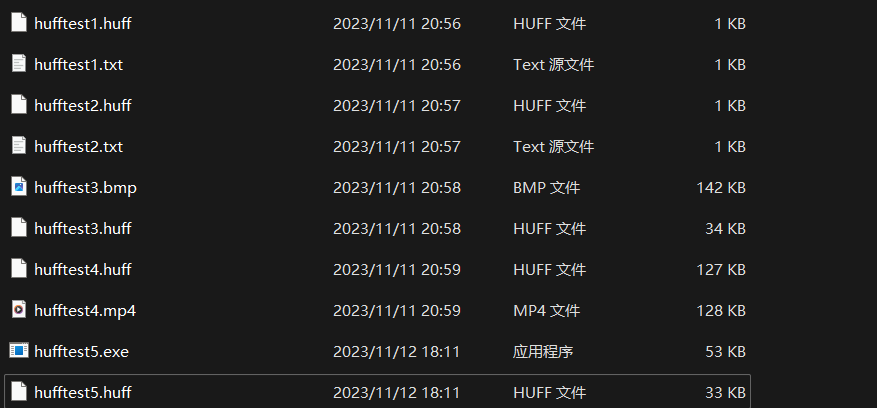
\includegraphics[height=6cm,width=12cm]{2.png}
		\end{figure}
	2\_1.txt压缩率为54.1\%;
	
	2\_2.txt压缩率为70.1\%;

	2\_3.bmp压缩率为23.7\%;
	
	2\_4.mp4压缩率为99.6\%;
	
	2\_5.exe压缩率为60.5\%。
	\section{实验体会收获}

通过本次实验运用了二叉树的相关性质,
掌握了霍夫曼编码的原理和实现方法,并实现了对文件的压缩和解压缩操作,同时复习了文件相关操作。
   
\end{document}